%Report writing
\documentclass [12pt] {report}

%import packages
%for bullets
\usepackage{enumerate}
%for maths formulae
\usepackage{amsmath}
%for table
\usepackage{longtable}
%for repositioning
\usepackage{float}
%for figure insertion
\usepackage{graphicx}

%set page margins
\setlength {\topmargin} {-2cm}
\setlength {\oddsidemargin} {0cm}
\setlength {\textheight} {24cm}
\setlength {\textwidth} {16cm}

%declare title and authors
\title{\textbf{Manually Operated Cashew Nut Segregation and Shelling Machine}}
\author{Agro-Mechanical Project\\\\A. Takawale, V. Swakul, S.Tripathi, A. Vipradas} 

%begin document
\begin{document}

%make lists
\maketitle
\tableofcontents
\listoffigures
\listoftables

%chapter: introduction
\chapter{Introduction}
The cashew fruit, \textit{(Anacardium occidentale)}, belongs to the Anacardiaceae family. The name Anacardium refers to the shape of the fruit which looks like an inverted \textit{heart}. The cashew tree is small and evergreen, growing 10-12m tall, with a short, often irregularly shaped trunk. The true fruit of the cashew tree is a kidney or boxing-glove shaped drupe that grows at the end of a cashew apple.\\Nigeria was the world's largest producer of cashew nuts with shell in 2010 with a yield of 1.97 MT/hectare followed by Vietnam(0.85), India(0.66) and Ivory Coast(0.44). Vietnam overtook Nigeria as the largest producer in 2012.\\According to the statistics of India in 2009-10, Maharashtra was the leading producer and processor of cashew nuts with average productivity of 1186 kg per hectare followed by Kerala(957) and West Bengal(909).\\In India, cashew nut is processed with the aid of manual and automatic shelling machines. Due to the intricacy and complexity of its shape, a cashew nut is to be shelled with utmost skill and care. A slight lack of judgement can damage the kernel inside the cashew nut. Barring a few, machines cannot compare human skill and judgement. That is why, the manual machines are preferred over the automatic shelling machines. The efficiency of a cashew nut shelling machine is defined as the total number of whole kernels obtained after 100 raw and roasted cashew nuts are shelled. The automatic machines deliver 90-92\% efficiency while the manual machines are 95\% efficient. Along with the efficiency, there are several other reasons for preferring manually operated shelling machines over automatic ones.\\The poverty and unemployment rate in India is very high. 29.8\% of the Indian population lives in poverty while 9.4\% are unemployed. According to government data, over 5,000 farmers committed suicide in 2005-2009 in Maharashtra. In order to improve the economy of India it is very important to harness the manual labour in order to decrease the unemployment rate. Employment of the unemployed also results in their fulfillment of basic needs. This is another reason why the manual shelling machines are preferred over the automatic shelling machines.\\There is a tremendous variation in the size and dimensions of cashew nuts. The shell thickness of cashew nuts decrease with their size. Thus, shelling of small cashew nuts pose a big problem during the cashew nut shelling process consequently reducing its overall efficiency. Worker operated machines prove to be more efficient as compared to the automatic machines as far as shelling of small cashew nuts is concerned. This has compelled most of the industries to adopt manually operated machines over automatic machines. Even though the manual machines are more efficient while shelling small cashew nuts, the whole kernel recovery for these is very low.\\Cost is another factor responsible for the use of manually operated machines on a large scale. While an automatic shelling machine costs 65000Rs,  a manually operated machine is available only for 2500Rs.\\Just as the automatic shelling machines have their disadvantages, the manually operated machines have theirs. A laborer working on a manually operated shelling machine is required to hold the cashew nut in his hand while piercing the cashew nut shell with the knife blade. This poses a great risk towards the safety of the laborer especially while shelling small cashew nuts. There is a high chance of the worker cutting his thumb or index finger. As safety of the worker is of utmost importance and prime concern, it is the need to design and manufacture a shelling machine which ensures safety and efficiently shells small cashew nuts at the same time.\\The currently used manually operated machines can only be operated by skilled workforce. Generally farmers producing cashew nuts are unskilled in operating the shelling machines. Due to the presence of middlemen who process and shell cashew nuts, it is these people who earn a lot of money leaving a very minor share for farmers. The cost of processed and shelled cashew nuts of W-180 grade is around 700Rs per kg while that of raw cashew nuts which a farmer sells to the processing industry is merely 10Rs per kg. It would be very beneficial and profitable for the farmer if he is able to process the cashew nuts on his own right after its production. Considering all these factors, it is the need of the hour to manufacture a cashew nut shelling machine which ensures safety, shells all sizes of cashew nuts, can be used by any unskilled person and has the efficiency and cost at par with the currently used manually operated commercial shelling machines.

%bibliography remaining !!!!!
\section{References}
http://en.wikipedia.org/wiki/Cashew\\
http://en.wikipedia.org/wiki/Economy\_of\_India\\
http://www.rawcashewnuts.com/Commercial-info.html\\
http://en.wikipedia.org/wiki/Farmers'\_suicides\_in\_India\\
http://www.buddhiindustry.lk/index.php\\
http://dccd.gov.in/stat.htm\#top\\

%chapter : design of scotch-yoke mechanism
\chapter{Design of the scotch-yoke mechanism}

%start bullets (roman)
\begin{enumerate}[I]
\item
\textbf{\textit{Fluctuating compressive load on the yoke during cashew nut shear}}

%table
\begin{longtable}{|l|l|l|l|l|}
\caption{Calculations for cross-section of the yoke}\\
\hline 
\textbf{Parameter} & \textbf{Symbol} & \textbf{Formula} & \textbf{Value} & \textbf{Unit}\\
\hline
\hline
Ultimate tensile strength of yoke (MS) & \textit{$S_{ut}$} & - & 400 & MPa\\
\hline
Maximum force acting on the yoke & \textit{Pmax} & - & 300 & N\\ 
\hline
Minimum force acting on the yoke & \textit{Pmin} & - & 0 & N\\
\hline
Endurance strength of yoke & \textit{$S_e^{'}$} & $\textit{$S_{ut}$}/2$ & 200 & MPa\\
\hline
Surface finish factor(hot rolling) & \textit{$K_a$} & - & 0.8 & -\\
\hline
Size factor ($<$ 7.5 mm) &  \textit{$K_b$} & - & 1 & -\\
\hline
Reliability factor (99 percent) &  \textit{$K_c$} & - & 0.814 & -\\
\hline
Account stress concentration (notch free) &  \textit{$K_d$} & - & 1 & -\\
\hline
Corrected endurance strength & $S_e$ &  \textit{$K_a$}  \textit{$K_b$}  \textit{$K_c$} \textit{$K_d$} \textit{$S_e^{'}$} & 130.24 & MPa \\
\hline
Mean force on the yoke & \textit{Pm} & $(\textit{Pmax} + \textit{Pmin})/2$ & 150 & N\\
\hline
Force amplitude on the yoke  & \textit{Pa} & $(\textit{Pmax} - \textit{Pmin})/2$ & 150 & N\\
\hline
Theta on modified goodman diagram & \textit{$\theta$} & $tan^{-1}(\textit{Pa}/\textit{Pm})$ & 45 & degree\\
\hline
Stress amplitude (refer Figure \ref{fig:goodman1}) & \textit{$S_a$} & $( \textit{$S_{ut}$} \textit{$S_e$})/( \textit{$S_{ut}$} +  \textit{$S_e$})$ & 98.25 & MPa\\
\hline
Factor of safety & \textit{fs} & - & 2 & -\\
\hline
\textbf{c/s of yoke} & \textit{A} & $(\textit{Pa}* \textit{fs})/2$ &\textbf{3.053} & $mm^2$\\
\hline
\textbf{Assumed c/s of yoke} & \textit{A} & - & \textbf{15 x 5} & $mm^2$\\
\hline
\end{longtable}

%figure
\begin{figure}[H]
\begin{center}
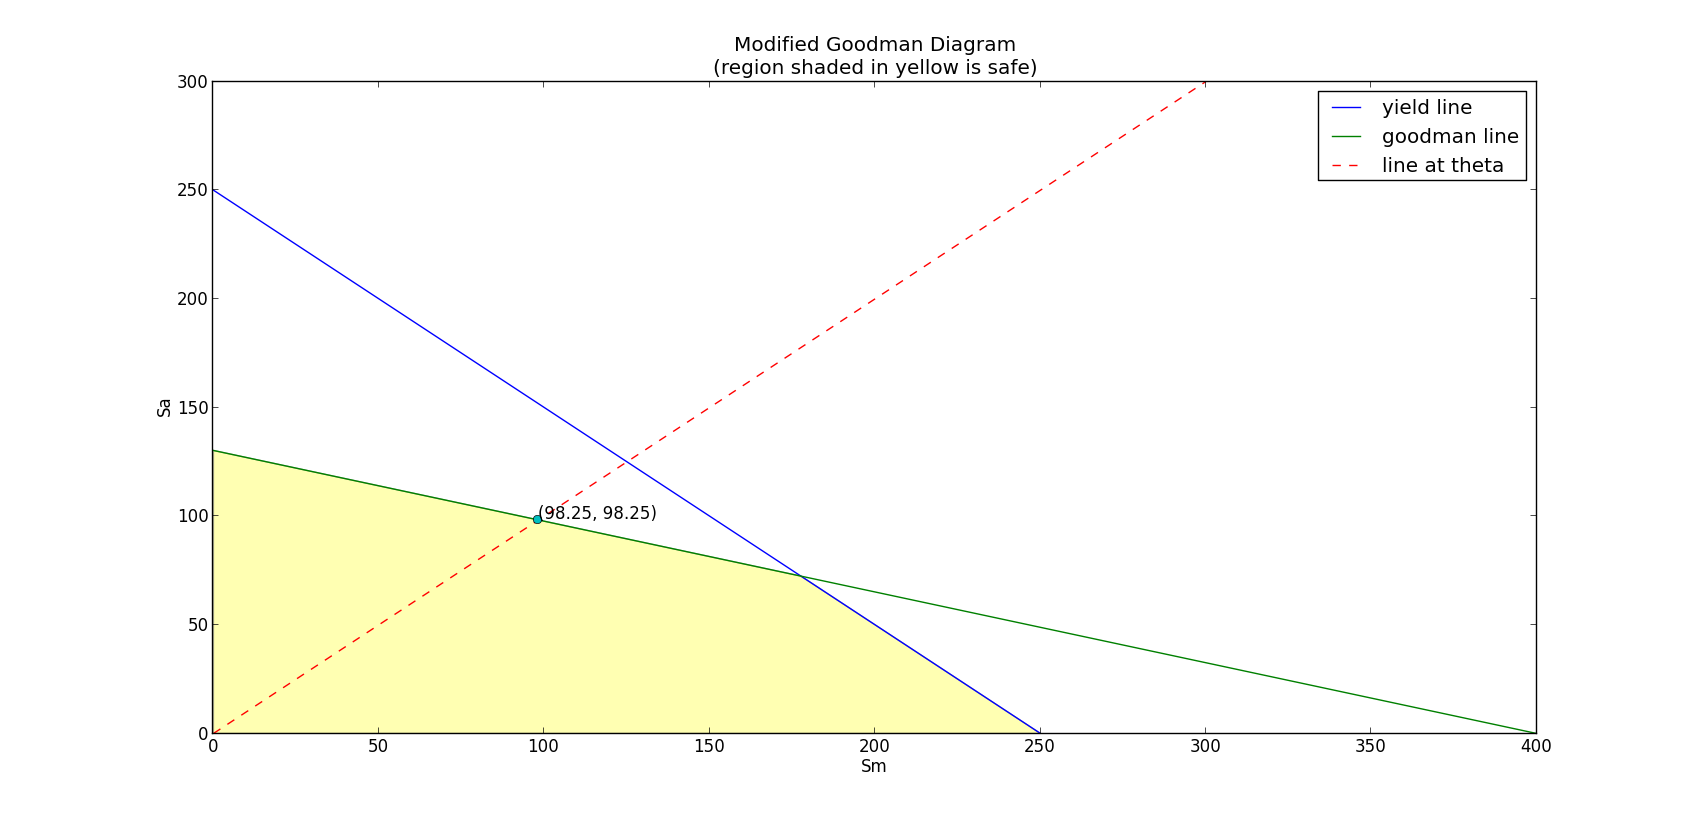
\includegraphics[width=7in,height=4in]{goodman1.png}
\caption{Modified goodman diagram for c/s of yoke}
\label{fig:goodman1}
\end{center}
\end{figure}

\item
\textbf{\textit{Fluctuating compressive load on yoke and slot weld}}

%table
\begin{longtable}{|l|l|l|l|l|}
\caption{Calculations for cross-section of the weld between yoke and slot}\\
\hline 
\textbf{Parameter} & \textbf{Symbol} & \textbf{Formula} & \textbf{Value} & \textbf{Unit}\\
\hline
\hline
Ultimate tensile strength of weld & \textit{$S_{ut}$} & - & 450 & MPa\\
\hline
Maximum force acting on the weld & \textit{Pmax} & - & 300 & N\\ 
\hline
Minimum force acting on the weld & \textit{Pmin} & - & 0 & N\\
\hline
Endurance strength of weld & \textit{$S_e^{'}$} & $\textit{$S_{ut}$}/2$ & 225 & MPa\\
\hline
Surface finish factor(low surface finish) & \textit{$K_a$} & - & 0.52 & -\\
\hline
Size factor ($<$ 7.5 mm) &  \textit{$K_b$} & - & 1 & -\\
\hline
Reliability factor (99 percent) &  \textit{$K_c$} & - & 0.814 & -\\
\hline
Fatigue factor(Reinforced butt-weld) & \textit{$K_f$} & - & 1.2 &-\\
\hline
Account stress concentration (notch free) &  \textit{$K_d$} & $1/\textit{$K_d$}$ & 0.833 & -\\
\hline
Corrected endurance strength & $S_e$ &  \textit{$K_a$}  \textit{$K_b$}  \textit{$K_c$} \textit{$K_d$} \textit{$S_e^{'}$} & 79.33 & MPa \\
\hline
Mean force on the weld & \textit{Pm} & $(\textit{Pmax} + \textit{Pmin})/2$ & 150 & N\\
\hline
Force amplitude on the weld  & \textit{Pa} & $(\textit{Pmax} - \textit{Pmin})/2$ & 150 & N\\
\hline
Theta on modified goodman diagram & \textit{$\theta$} & $tan^{-1}(\textit{Pa}/\textit{Pm})$ & 45 & degree\\
\hline
Stress amplitude (refer Figure \ref{fig:goodman2}) & \textit{$S_a$} & $( \textit{$S_{ut}$} \textit{$S_e$})/( \textit{$S_{ut}$} +  \textit{$S_e$})$ &67.44 & MPa\\
\hline
Factor of safety & \textit{fs} & - & 2 & -\\
\hline
\textbf{c/s of weld $<$(15 x 5)} & \textit{A} & $(\textit{Pa}* \textit{fs})/2$ &\textbf{4.448} & $mm^2$\\
\hline
\end{longtable}

%figure
\begin{figure}[H]
\begin{center}
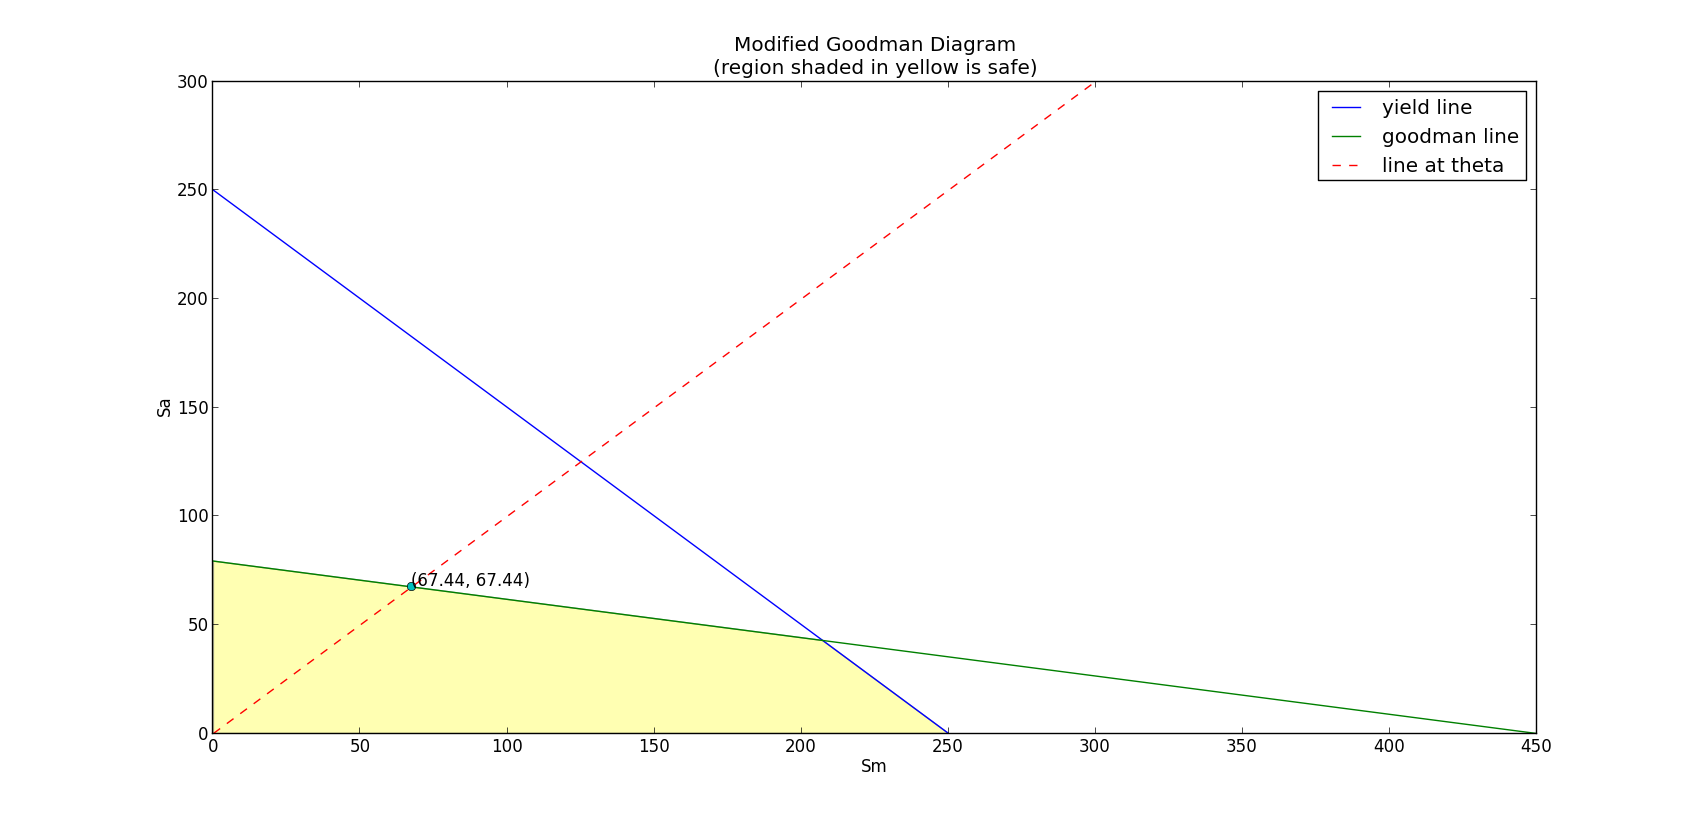
\includegraphics[width=7in,height=4in]{goodman2.png}
\caption{Modified goodman diagram for c/s of yoke-slot weld}
\label{fig:goodman2}
\end{center}
\end{figure}

\item
\textbf{\textit{Shear force and torsion on yoke-slot weld}}

%table
\begin{longtable}{|l|l|l|l|l|}
\caption{Calculations for width of yoke-slot weld}\\
\hline 
\textbf{Parameter} & \textbf{Symbol} & \textbf{Formula} & \textbf{Value} & \textbf{Unit}\\
\hline
\hline
Surface area of both the welds & \textit{A} & - & - & $mm^2$ \\
\hline
Maximum shear load on the welds & \textit{P} & - & 300 & N\\
\hline
Eccentricity & \textit{e} & - & 90 & mm\\
\hline
Primary shear stress & $\tau_1$ & $\textit{P/A}$ & $300/\textit{A}$ & $N/mm^2$\\ 
\hline
Distance between system C.G. and weld C.G  & \textit{d} & - & 90 & mm\\
\hline
Half the length of weld (c/s 15 x 5) & \textit{c} & $15/2$ & 7.5 & mm\\
\hline
Maximum distance between system C.G. and weld & \textit{r} & $\sqrt{d^2 + c^2}$ & 90.31 & mm\\
\hline
Maximum moment on the welds & \textit{$M_t$} & \textit{Pe} & 27000 & N-mm\\
\hline
Polar moment of inertia of the weld system & \textit{J} & $2A(l^2/12 + R^2)$ & 16237.5A & $mm^4$\\
\hline
Secondary shear stress & $\tau_2$ & \textit{$M_t$}\textit{$r/J$}& $150.17/A$ & $N/mm^2$\\
\hline
Permissible shear stress & $\tau$ & - & 100 & $N/mm^2$\\
\hline
Width of both the welds & \textit{w} & $\textit{res}/\tau$ & 0.231 & mm\\
\hline 
\end{longtable}

%end bullets
\end{enumerate}

%end document
\end{document}
